
\documentclass[10pt]{standalone}
\input{../../tikzpic_packages.tex}
\begin{document}
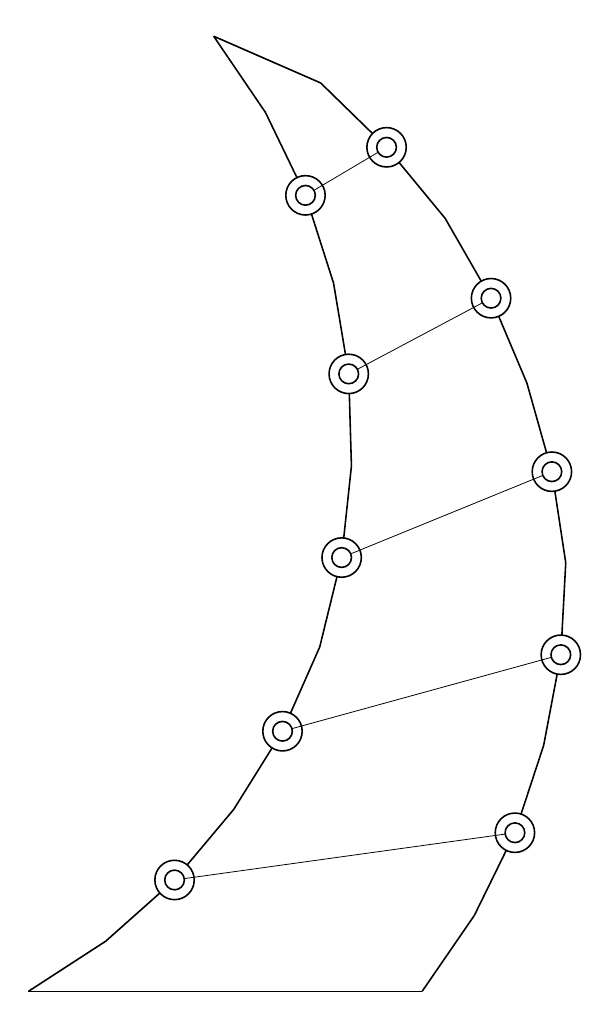
\begin{tikzpicture}
\tikzset{
    scale=5,
    part/.style={line width = .2mm, color=black},
    joint/.style={line width = .2mm, color=black, fill=white},
    grid line/.style={gray},
    link/.style={line width=.1mm, color=black}
    }

\draw[part] (-0.500000, 0.000000) coordinate(Llast) -- (0.500000, 0.000000) coordinate(Rlast);

\path (-0.303708, 0.127292) coordinate(L) -- (0.632575, 0.192763) coordinate(R);
\draw[part] (L)--(Llast) (R)--(Rlast);
\path (L)coordinate(Llast) (R)coordinate(Rlast);
\path (-0.128941, 0.282824) coordinate(L) -- (0.735646, 0.402787) coordinate(R);
\draw[part] (L)--(Llast) (R)--(Rlast);
\path (L)coordinate(Llast) (R)coordinate(Rlast);
\path (0.021407, 0.462070) coordinate(L) -- (0.808716, 0.625036) coordinate(R);
\draw[part] (L)--(Llast) (R)--(Rlast);

\draw[joint] (Llast)circle(.05);
\draw[joint] (Rlast)circle(.05);
\draw[link] (Llast)--(Rlast);
\draw[joint] (Llast)circle(.025);
\draw[joint] (Rlast)circle(.025);
\path (L)coordinate(Llast) (R)coordinate(Rlast);
\path (0.145250, 0.660555) coordinate(L) -- (0.852215, 0.854909) coordinate(R);
\draw[part] (L)--(Llast) (R)--(Rlast);
\path (L)coordinate(Llast) (R)coordinate(Rlast);
\path (0.239808, 0.874548) coordinate(L) -- (0.864735, 1.088526) coordinate(R);
\draw[part] (L)--(Llast) (R)--(Rlast);

\draw[joint] (Llast)circle(.05);
\draw[joint] (Rlast)circle(.05);
\draw[link] (Llast)--(Rlast);
\draw[joint] (Llast)circle(.025);
\draw[joint] (Rlast)circle(.025);
\path (L)coordinate(Llast) (R)coordinate(Rlast);
\path (0.295518, 1.101770) coordinate(L) -- (0.829535, 1.319815) coordinate(R);
\draw[part] (L)--(Llast) (R)--(Rlast);
\path (L)coordinate(Llast) (R)coordinate(Rlast);
\path (0.320356, 1.334400) coordinate(L) -- (0.766054, 1.544990) coordinate(R);
\draw[part] (L)--(Llast) (R)--(Rlast);

\draw[joint] (Llast)circle(.05);
\draw[joint] (Rlast)circle(.05);
\draw[link] (Llast)--(Rlast);
\draw[joint] (Llast)circle(.025);
\draw[joint] (Rlast)circle(.025);
\path (L)coordinate(Llast) (R)coordinate(Rlast);
\path (0.313511, 1.568253) coordinate(L) -- (0.675003, 1.760498) coordinate(R);
\draw[part] (L)--(Llast) (R)--(Rlast);
\path (L)coordinate(Llast) (R)coordinate(Rlast);
\path (0.274896, 1.798996) coordinate(L) -- (0.558403, 1.963323) coordinate(R);
\draw[part] (L)--(Llast) (R)--(Rlast);

\draw[joint] (Llast)circle(.05);
\draw[joint] (Rlast)circle(.05);
\draw[link] (Llast)--(Rlast);
\draw[joint] (Llast)circle(.025);
\draw[joint] (Rlast)circle(.025);
\path (L)coordinate(Llast) (R)coordinate(Rlast);
\path (0.203643, 2.021834) coordinate(L) -- (0.409608, 2.143861) coordinate(R);
\draw[part] (L)--(Llast) (R)--(Rlast);
\path (L)coordinate(Llast) (R)coordinate(Rlast);
\path (0.101890, 2.232500) coordinate(L) -- (0.242181, 2.307268) coordinate(R);
\draw[part] (L)--(Llast) (R)--(Rlast);

\draw[joint] (Llast)circle(.05);
\draw[joint] (Rlast)circle(.05);
\draw[link] (Llast)--(Rlast);
\draw[joint] (Llast)circle(.025);
\draw[joint] (Rlast)circle(.025);
\path (L)coordinate(Llast) (R)coordinate(Rlast);
\path (-0.029620, 2.425991) coordinate(L) -- (0.055016, 2.447635) coordinate(R);
\draw[part] (L)--(Llast) (L)--(Rlast);
\path (L)coordinate(Llast) (R)coordinate(Rlast);
%\draw[part] (L)--(R);
\end{tikzpicture}
\end{document}
